%%
%% This is file `sample-manuscript.tex',
%% generated with the docstrip utility.
%%
%% The original source files were:
%%
%% samples.dtx  (with options: `manuscript')
%% 
%% IMPORTANT NOTICE:
%% 
%% For the copyright see the source file.
%% 
%% Any modified versions of this file must be renamed
%% with new filenames distinct from sample-manuscript.tex.
%% 
%% For distribution of the original source see the terms
%% for copying and modification in the file samples.dtx.
%% 
%% This generated file may be distributed as long as the
%% original source files, as listed above, are part of the
%% same distribution. (The sources need not necessarily be
%% in the same archive or directory.)
%%
%% The first command in your LaTeX source must be the \documentclass command.
\documentclass[manuscript,screen,review]{acmart}

%%
%% \BibTeX command to typeset BibTeX logo in the docs
\AtBeginDocument{%
  \providecommand\BibTeX{{%
    \normalfont B\kern-0.5em{\scshape i\kern-0.25em b}\kern-0.8em\TeX}}}

%% Rights management information.  This information is sent to you
%% when you complete the rights form.  These commands have SAMPLE
%% values in them; it is your responsibility as an author to replace
%% the commands and values with those provided to you when you
%% complete the rights form.

%% These commands are for a PROCEEDINGS abstract or paper.

\def\@copyrightspace{\relax}
%%
%% Submission ID.
%% Use this when submitting an article to a sponsored event. You'll
%% receive a unique submission ID from the organizers
%% of the event, and this ID should be used as the parameter to this command.
%%\acmSubmissionID{123-A56-BU3}

%%
%% The majority of ACM publications use numbered citations and
%% references.  The command \citestyle{authoryear} switches to the
%% "author year" style.
%%
%% If you are preparing content for an event
%% sponsored by ACM SIGGRAPH, you must use the "author year" style of
%% citations and references.
%% Uncommenting
%% the next command will enable that style.
%%\citestyle{acmauthoryear}

%%
%% end of the preamble, start of the body of the document source.
\begin{document}

%%
%% The "title" command has an optional parameter,
%% allowing the author to define a "short title" to be used in page headers.
\title{Do solutions for catastrophic forgetting degrade model robustness to naturalistic corruption and adversarial attacks?}

%%
%% The "author" command and its associated commands are used to define
%% the authors and their affiliations.
%% Of note is the shared affiliation of the first two authors, and the
%% "authornote" and "authornotemark" commands
%% used to denote shared contribution to the research.
\author{Tuan Pham}
\email{tuanph18@uchicago.edu}
\affiliation{%
  \institution{The University of Chicago}
  \city{Chicago}
  \state{Illinois}
  \country{USA}
}

\author{Amit Pradhan}
\email{pradhanak@uchicago.edu}
\affiliation{%
  \institution{The University of Chicago}
  \city{Chicago}
  \state{Illinois}
  \country{USA}
}

\author{Sebastian Barrios}
\email{sebastian.barrios@chicagobooth.edu}
\affiliation{%
  \institution{The University of Chicago}
  \city{Chicago}
  \state{Illinois}
  \country{USA}
}


%%
%% By default, the full list of authors will be used in the page
%% headers. Often, this list is too long, and will overlap
%% other information printed in the page headers. This command allows
%% the author to define a more concise list
%% of authors' names for this purpose.
%% TO-DO
%%
%% The abstract is a short summary of the work to be presented in the
%% article.
%% TO-DO
\begin{abstract}
  \textbf{Insert ABSTRACT here}
\end{abstract}

%%
%% The code below is generated by the tool at http://dl.acm.org/ccs.cfm.
%% Please copy and paste the code instead of the example below.
%%

%% TO-DO
\begin{CCSXML}
<ccs2012>
 <concept>
  <concept_id>10010520.10010553.10010562</concept_id>
  <concept_desc>Computer systems organization~Embedded systems</concept_desc>
  <concept_significance>500</concept_significance>
 </concept>
 <concept>
  <concept_id>10010520.10010575.10010755</concept_id>
  <concept_desc>Computer systems organization~Redundancy</concept_desc>
  <concept_significance>300</concept_significance>
 </concept>
 <concept>
  <concept_id>10010520.10010553.10010554</concept_id>
  <concept_desc>Computer systems organization~Robotics</concept_desc>
  <concept_significance>100</concept_significance>
 </concept>
 <concept>
  <concept_id>10003033.10003083.10003095</concept_id>
  <concept_desc>Networks~Network reliability</concept_desc>
  <concept_significance>100</concept_significance>
 </concept>
</ccs2012>
\end{CCSXML}

\ccsdesc[500]{Computer systems organization~Embedded systems}
\ccsdesc[300]{Computer systems organization~Redundancy}
\ccsdesc{Computer systems organization~Robotics}
\ccsdesc[100]{Networks~Network reliability}

%%
%% Keywords. The author(s) should pick words that accurately describe
%% the work being presented. Separate the keywords with commas.
\keywords{datasets, neural networks, gaze detection, text tagging}


%%
%% This command processes the author and affiliation and title
%% information and builds the first part of the formatted document.
\maketitle

\section{Introduction}
Developing a deep learning model, for example in image classification, is not only about achieving the best classification accuracy. Even with increasing computational power, there are multiple issues that also need to be solved, including - to name a few - fast inference time, manageable memory size, continual learning and robustness to data/model corruption. An attractive solution for fast computation, efficient power consumption and potentially easier hardware implementation is binary neural networks (BNN) \cite{DBLP:journals/corr/CourbariauxB16}, in which only the signs of the model’s hidden weights are utilized during inference. 

A recent study takes inspiration from biological metaplasticity to solve catastrophic forgetting (CF) problems and continual learning problems for BNN \cite{Laborieux_Ernoult_Hirtzlin_Querlioz_2021}. More specifically, by creating a form of multiplicative gating during learning for hidden weights to represent weight consolidation, they are able to solve the permuted-MNIST task, sequential learning with CIFAR-10/100 dataset, and stream learning with these datasets. This approach shares certain similarities with another study in regular neural networks, also inspired by neuroscience literature, which takes into account (a) weight stabilization based on task importance, combined with (b) context-dependent gating allowing for more sparse, non-overlapping population activations, to facilitate learning and remembering a large number of tasks \cite{Masse_2018}. 

Back to BNNs, due to such quantization, they can be quite sensitive to corruption, for example data adversarial attacks \cite{Lin_2019} or potential soft errors in hardware accelerators \cite{Khoshavi2020}. Hence, we wish to ask whether previous solutions for CF \cite{Laborieux_Ernoult_Hirtzlin_Querlioz_2021} could further degrade model robustness to data corruption or help ameliorate it.

In conclusion, we propose a plan to (i) replicate the selected studies that tackle the topic of catastrophic forgetting, and (ii) observe whether solutions to avoid CF lead to models that have a higher level of degradation when different types of naturalistic corruption to input data are introduced \cite{Hendrycks_2018}, as well as the potential resulting vulnerability of these models to adversarial attacks \cite{Lin_2019}.

%% TO-DO
\section{Methods}
The specific methods will be discussed in detail later. Code repository currently at: 
\url{https://github.com/tuanpham96/bnn-cf-vs-robust}

\section{(Initial) Results}
\subsection{Experiment 0: Replication of BNN training with metaplasticity parameter with permuted MNIST
}

Before applying corruptions to the dataset, we first set out to observe whether the original results from \cite{Laborieux_Ernoult_Hirtzlin_Querlioz_2021} were replicable. So we ran their codes for the multipercepton (MLP) version of the BNN with 2 hidden layers (1024 units each) for different values of the meta hyperparameters: low meta means binary hidden weights are allowed to change easily while high means such weights’ own plasticity is constrained by their magnitude. This is shown in Fig. 1b. Consistent with the paper, higher meta leads to better performance (potentially criticality is around 1.0), in which earlier tasks still perform well. Interestingly, too high value 2.0) might lead to performing not as well (though still good) for the current task - this is basically because high values would bias most changes happening for earlier tasks and would require longer time to learn the current task. Regardless, these results confirm the benefits of the metaplasticity to solve the permuted MNIST task, which is one of the benchmarks for catastrophic forgetting. 

Additionally, we also try to replicate the relationship between the sizes of the hidden layers and the performance (Fig. \ref{fig:fig1}c). Contrary to the monotonic trend between the trend and the performance shown in the original paper, we found that large networks could be harmful. For now, we are unsure why. One of the reasons might be that we only allowed for 20 epochs per task for this benchmark while the original paper allowed for 40 epochs. Maybe larger networks require a bit more time to consolidate properly. We might run our training again with the exact same hyperparameter settings to see whether it might just have been some nuances in the settings. 

\begin{figure}[h]
    \centering
    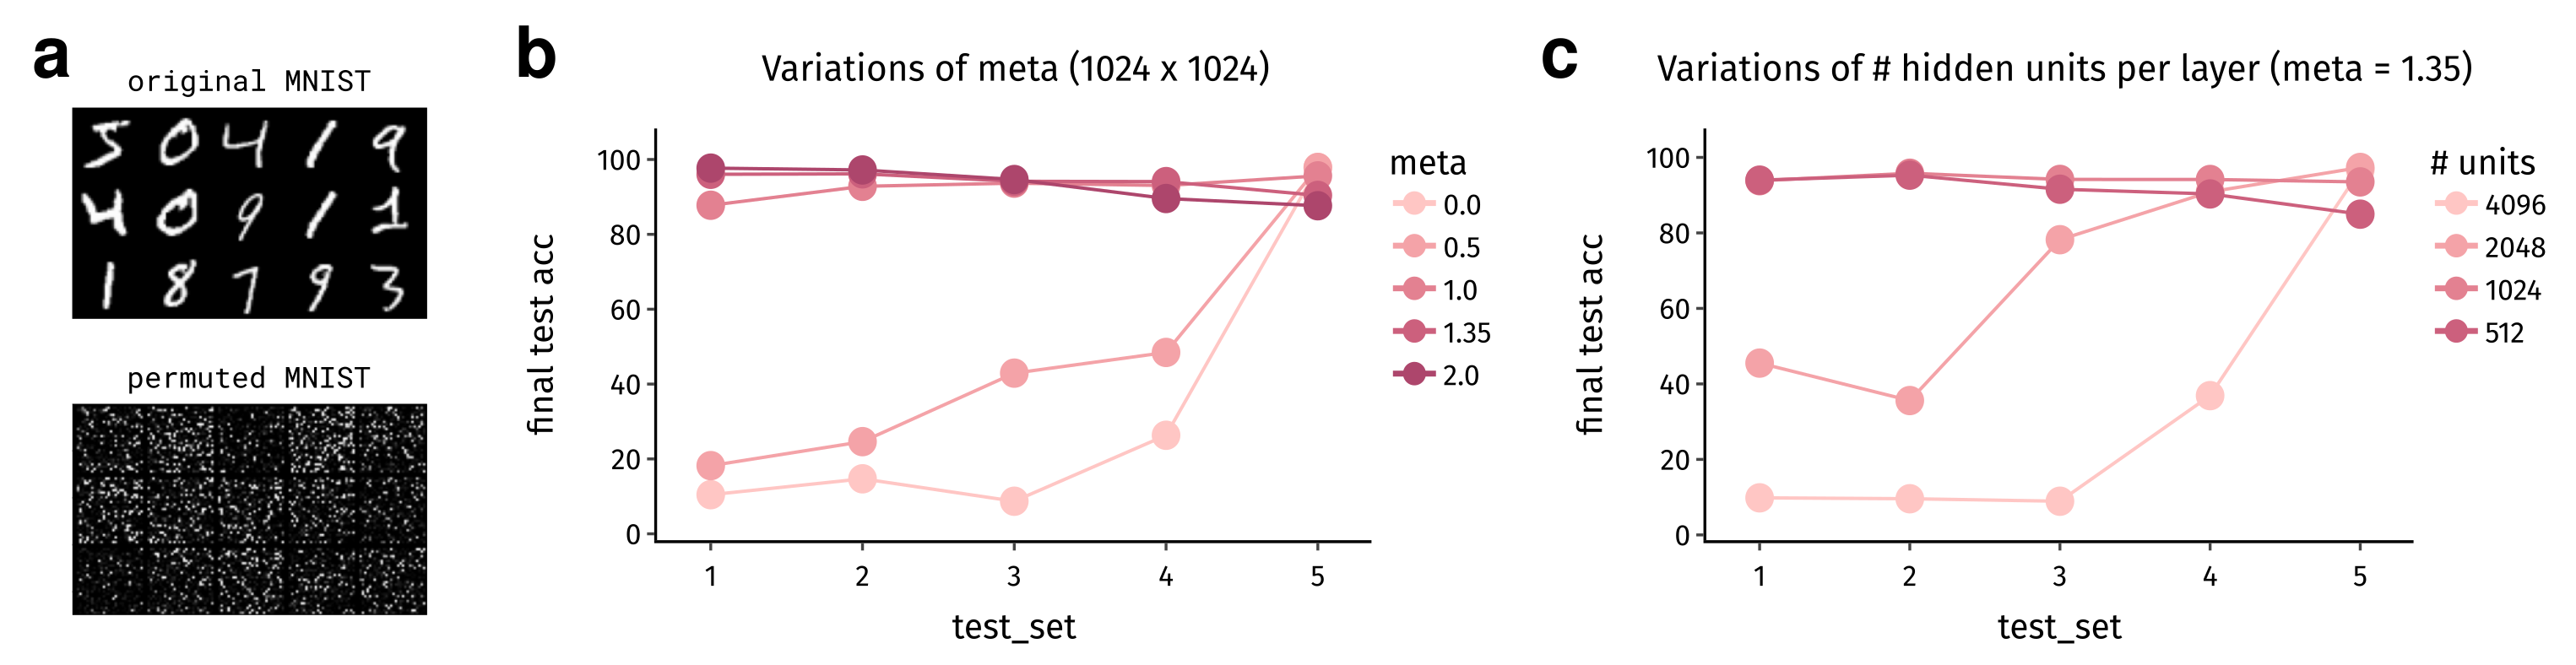
\includegraphics[width=0.9\textwidth]{figures/report/Fig1.png}
    \caption{Results of permuted MNIST tasks for the BNNs with metaplasticity training. (a) Example of original (top, task 1) and generated permuted (bottom, after task 1) MNIST dataset. (b) Performance of the BNN (MLP, 2 hidden layers, 1024 units each) with different values of metaplasticity hyperparameter (c) Performance with variations in the number of hidden units per layer with meta = 1.35}
    \label{fig:fig1}
\end{figure}

\subsection{Experiment 1.1: Metaplasticity-trained BNN in response to natural corruptions to pMNIST tasks 
}

\begin{figure}[ht]
    \centering
    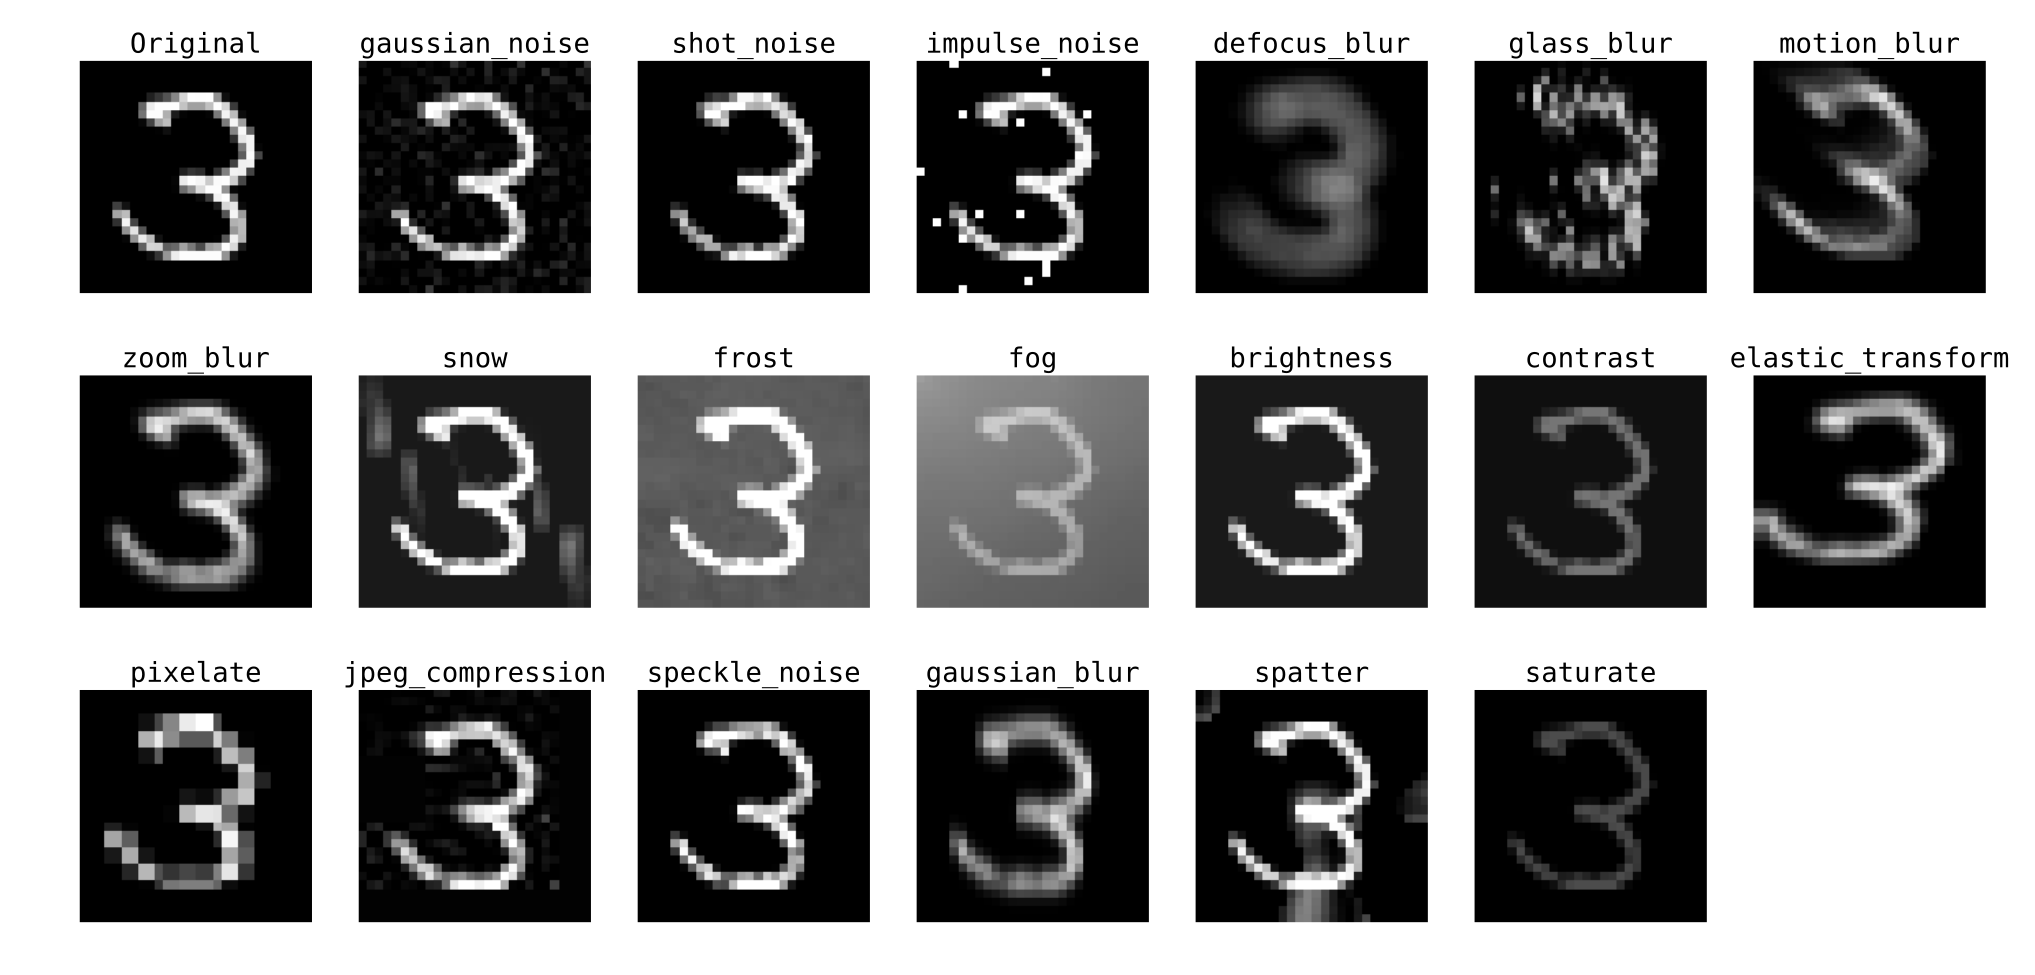
\includegraphics[width=0.9\textwidth]{figures/report/Fig2.png}
    \caption{Examples of the natural corruptions for MNIST data, plotted with similar color limits}
    \label{fig:fig2}
\end{figure}

Next we moved on to applying perturbations onto our MNIST and pMNIST datasets after training the BNN models with metaplasticity optimization. First, we modified the code from \cite{Hendrycks_2018} to allow for monochrome natural corruptions on our (p)MNIST datasets. Because some of these transformations are not easily standardized for tensor transformation, these corrupted data sets are pre-generated before training, to save time during testing. The examples of these corruption transformations are shown in Fig. \ref{fig:fig2}. It must be noted that these types of corruption are possibly more realistic when considered with colored images like CIFAR or ImageNet, and the more appropriate benchmarks for catastrophic forgetting coupled with these types of perturbations would be MNIST-FashMNIST or split-class CIFAR. Regardless, for now we chose permuted MNIST as our first approach to assess catastrophic forgetting with natural corruptions.

The results are shown in Fig. \ref{fig:fig3} for the models at the end of training for different values of meta, tested for the original (last panel) test data sets of all tasks (i.e. task data source) and the natural corruptions shown in Fig. \ref{fig:fig2}. For many different perturbations (for example brightness or shot\_noise, impulse\_noise), at least the inclusion of the metaplasticity training seems to help safeguard the model against the corruption for earlier tasks, though there’s not a consistent trend for the actual magnitude of meta. At the same time, for many of these transformations, no improvement is observed regardless. It must be noted that these models are 2048 x 2048, in which Fig. 1c already shows that this particular setting is not optimal. Hence, we would need to rerun this with more variations of the sizes just to be certain. 


\begin{figure}[h]
    \centering
    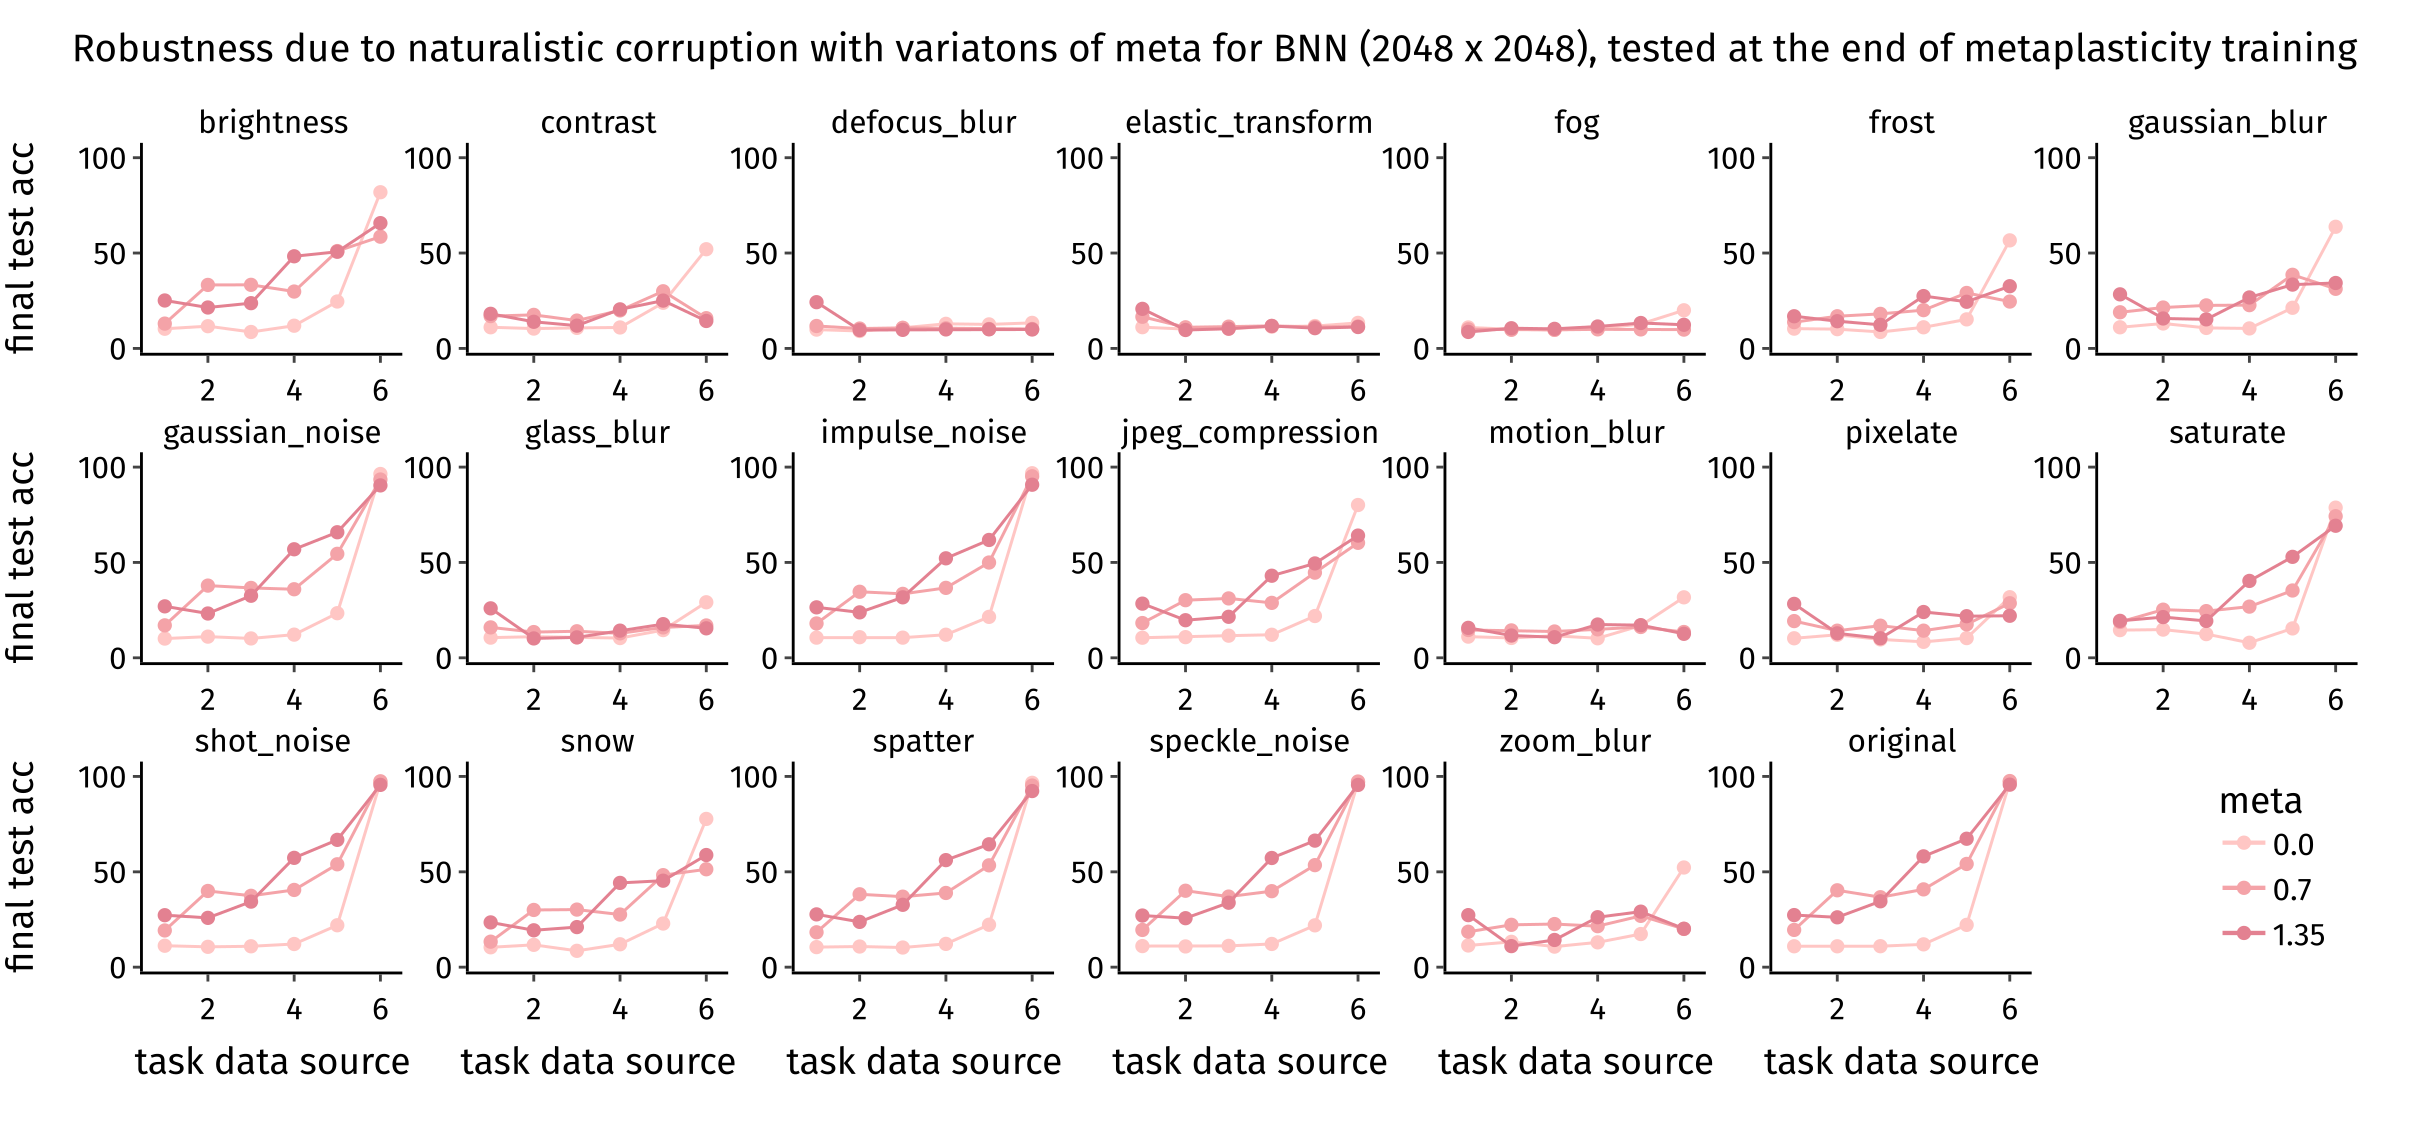
\includegraphics[width=0.9\textwidth]{figures/report/Fig3.png}
    \caption{Test performance of the BNN models at the end of metaplasticity (colors) training in response to different monochrome natural corruptions (panels, original is last) generated from different tasks. The model here is MLP BNN with 2 hidden layers of 2048 units each. See Fig \ref{fig:fig2}. for demonstrations of natural corruption. The x-axis for each panel represents where the original test data come from, e.g. task-2 in the shot\_noise panel means that the test dataset is the task-2 (permuted MNIST) that gets corrupted with shot\_noise corruption. }
    \label{fig:fig3}
\end{figure}


\subsection{Experiment 1.2: Metaplasticity-trained BNN in response to adversarial attacks to original MNIST data}

We have reproduced the effectiveness of a white-box adversarial attack ‘Fast Gradient Sign Attack (FGSM)’ with the goal of misclassification on BNN. Adversarial attacks in general try to add the least amount of perturbations to the input data to cause the desired misclassification. FGSM is a very powerful yet intuitive attack. For a given input, FGSM calculates the gradients of the loss function with respect to the input and adjusts the input by adding a small perturbation in the directions of the gradients to cause the misclassification. 

Currently, we have only examined the attacks on the original MNIST dataset (i.e. task-01) with the models trained like above. The results are shown in Fig. 4 (some examples are shown in Fig. 5), illustrating that BNN is quite sensitive to adversarial attacks and continual learning worsens the performance significantly. The metaplasticity process does not seem to lead to much improvement to guard against FGSM attacks, potentially only very little for quite small perturbation strengths. However, we are unclear yet how accuracy could reach below chance here. Regardless, we would train the models again for appropriate sizes, as well as exploring smaller perturbation strengths (< 0.05) to see whether there are actually clear benefits even in this range. Additionally, we could consider integrating the Lipschitz regularization term for the hidden weight matrices, as proposed in [4], in addition to metaplasticity training to safeguard against such attacks; then we could test again for both catastrophic forgetting, naturalistic corruption and adversarial attacks. 

\begin{figure}
    \centering
    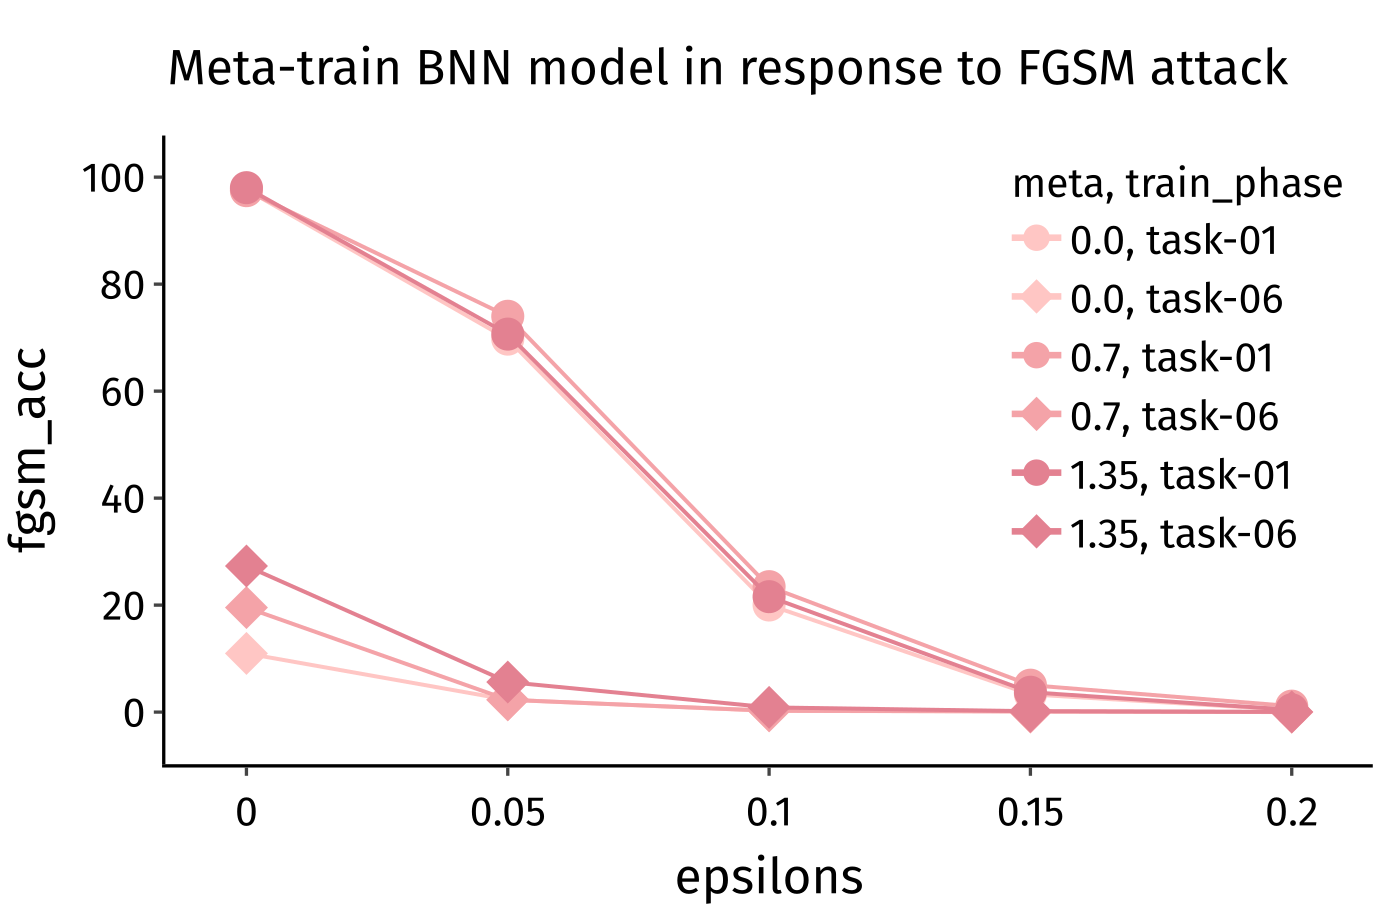
\includegraphics[width=0.9\textwidth]{figures/report/Fig4.png}
    \caption{FGSM adversarial attack on MNIST data of the BNN trained with metaplasticity during permuted MNIST task for 2 different training phases of the model. The test accuracy due to FGSM attacks is shown as a function of the perturbation strengths epsilons. Trained at task-01 refers to the end of the training phase in which the model was trained at MNIST dataset, while task-06 means that the model was the end of the entire metaplasticity training process. Only attacks on the original MNIST were tested here. Future iterations will integrate attacks on the following tasks (i.e. on pMNIST). }
    \label{fig:fig4}
\end{figure}

\section{Potential Next Steps}

In addition to (blue texts) re-running some of the trainings with a few more variations and re-testing on both natural corruptions, as well as adversarial attacks with FGSM with potential integration of Lipschitz regularization, here are a few other things we need to consider:
\begin{enumerate}
    \item Since the corruptions are more realistic for datasets such as CIFAR, we might need to start integrating the split-CIFAR with convolutional BNN, then re-apply these robustness tests.
    \item Measuring training times, memory and energy for the permuted MNIST tasks.
    \item Run one of the continuous-valued networks in the paper to have something to compare (2) with.
\end{enumerate}


%%
%% The next two lines define the bibliography style to be used, and
%% the bibliography file.
\bibliographystyle{ACM-Reference-Format}
\bibliography{bibliography}

%%
%% If your work has an appendix, this is the place to put it.
\appendix

\section{Research Methods}

\subsection{Part One}

Lorem ipsum dolor sit amet, consectetur adipiscing elit. Morbi
malesuada, quam in pulvinar varius, metus nunc fermentum urna, id
sollicitudin purus odio sit amet enim. Aliquam ullamcorper eu ipsum
vel mollis. Curabitur quis dictum nisl. Phasellus vel semper risus, et
lacinia dolor. Integer ultricies commodo sem nec semper.

\subsection{Part Two}

Etiam commodo feugiat nisl pulvinar pellentesque. Etiam auctor sodales
ligula, non varius nibh pulvinar semper. Suspendisse nec lectus non
ipsum convallis congue hendrerit vitae sapien. Donec at laoreet
eros. Vivamus non purus placerat, scelerisque diam eu, cursus
ante. Etiam aliquam tortor auctor efficitur mattis.

\section{Online Resources}

Nam id fermentum dui. Suspendisse sagittis tortor a nulla mollis, in
pulvinar ex pretium. Sed interdum orci quis metus euismod, et sagittis
enim maximus. Vestibulum gravida massa ut felis suscipit
congue. Quisque mattis elit a risus ultrices commodo venenatis eget
dui. Etiam sagittis eleifend elementum.

Nam interdum magna at lectus dignissim, ac dignissim lorem
rhoncus. Maecenas eu arcu ac neque placerat aliquam. Nunc pulvinar
massa et mattis lacinia.

\end{document}
\endinput
%%
%% End of file `sample-manuscript.tex'.
